% This is samplepaper.tex, a sample chapter demonstrating the
% LLNCS macro package for Springer Computer Science proceedings;
% Version 2.21 of 2022/01/12
%
\documentclass[runningheads]{llncs}
%
\usepackage[T1]{fontenc}
% T1 fonts will be used to generate the final print and online PDFs,
% so please use T1 fonts in your manuscript whenever possible.
% Other font encondings may result in incorrect characters.
%
\usepackage{graphicx}
% Used for displaying a sample figure. If possible, figure files should
% be included in EPS format.
%
% If you use the hyperref package, please uncomment the following two lines
% to display URLs in blue roman font according to Springer's eBook style:
%\usepackage{color}
%\renewcommand\UrlFont{\color{blue}\rmfamily}
%\urlstyle{rm}
%
% the environments 'definition', 'lemma', 'proposition', 'corollary',
% 'remark', and 'example' are defined in the LLNCS documentclass as well.
\usepackage{amsmath}

\begin{document}
%
\title{
Genetic Algorithm Search for Stable Vacua in Type IIB String Theory: A Computational Approach
}
\titlerunning{GA Search for Stable Vacua in Type IIB String Theory}
% --- SWITCH DE ANONIMATO ---
%\def\isanonymous{} 

\ifdefined\isanonymous
  \author{Anonymous Author(s)}
  \institute{Anonymous Organization\\ \email{anonymous@example.com}}
  \authorrunning{Anonymous et al.}
\else
  \author{Brandon Marquez-Salazar\inst{1} \and
  Cesar Damian\inst{1}\orcidID{0000-0003-4515-6570} \and
  Angel Diaz-Pacheco\inst{1}\orcidID{0000-0002-5978-0377}}
  \authorrunning{B. Marquez-Salazar et al.}
  \institute{División de Ingenierías Campus Irapuato-Salamanca, Universidad de Guanajuato, México \\
  \email{ba.marquezsalazar@ugto.mx}}
\fi

\maketitle              % typeset the header of the contribution
%
\begin{abstract}
%The abstract should briefly summarize the contents of the paper in
%150--250 words.

The exploration of high‑dimensional, non‑linear potential
landscapes is a central computational challenge. In fields
such as string theory, the search for stable vacuum
configurations reduces to a global optimisation problem on a
rugged objective function where classic grad\-ient‑based
methods are inadequate. Previous work demonstrated the
potential of nature‑inspired algorithms in this context.

In this work, a simple genetic algorithm (GA) is tailored to
the optimisation of a type IIB string theory potential with
torsion, extending the analysis of a previous work done with
Simulate Annealing (which found 203 stable dS and 529 stable
AdS). A penalty‑based objective enforces
critical point conditions, stability and a positive potential.
Using uniform bounds for the five flux coefficients and 100
independent runs, the GA explored the landscape extensively,
producing 11,979 critical points. The behaviour of the
potential under the $\widehat{D5}$ uplifting term was
analysed, revealing type transitions, modulus‑specific
effects and consistent negativity of $A_3\mathcal{N}_3$
without explicit constraints. The results confirm the GA’s
ability to discover stable de Sitter vacua and to provide a
rich dataset for further computational and theoretical study.

Finally, a grid was performed for the aim of finding better
configurations for this approach. The grid analysed 4
different models over 3 different moduli configurations.
The results were statistically analysed via fitness,
potential value and the amount of stable points found
(obtaining a stability ratio).

\keywords{Type IIB String Theory \and Flux Compactifications \and de Sitter Vacua \and Genetic Algorithms \and Global optimisation \and Metaheuristics}
\end{abstract}


%
\section{Introduction}

The exploration capabilities of computational nature‑inspired
methods have represented a significant advance in tackling
non‑linear models where traditional analytical or
gradient‑based techniques struggle \cite{Yang2020a,Ma2023}.
Among these, genetic algorithms (GA) stand out as a robust and
widely applicable metaheuristic. Inspired by natural selection,
GAs operate on populations of candidate solutions, evolving
them through selection, crossover, and mutation. This
population‑based approach enables effective exploration of
high‑dimensional, multimodal, and ill‑behaved solution spaces
without requiring convexity or differentiability assumptions
\cite{Yang2017,Eiben2015}. Consequently, GAs have become a
tool of choice for complex optimisation problems in
engineering and science.

In string theory, the exploration of the landscape—the set of
consistent vacuum configurations—poses a computational
challenge that exemplifies such difficulties. From an
optimisation standpoint, the problem reduces to finding minima
of a high‑dimensional potential energy function. The resulting
landscape is rugged: it contains numerous local optima,
strongly non‑convex regions, and numerical instabilities that
render deterministic methods ineffective \cite{Lanza2025,DeLuca2025}.
As the dimensionality and complexity of these models increase,
the need for robust, scalable computational tools becomes
critical \cite{Wilson2014}.

Recent work has demonstrated the potential of genetic
algorithms within this domain. \cite{Abel2014} showed that GAs
are orders of magnitude more efficient than random sampling for
locating viable string vacua. Hybrid approaches combining GAs
with neural networks have enabled the exploration of
exponentially larger spaces, yielding thousands of flux
configurations with critical points \cite{Bizet2020}. Beyond
efficiency, GAs have been shown to discover entirely new
configurations not present in exhaustive catalogs \cite{He2025},
highlighting their capacity for exploratory discovery.

A particularly relevant study by \cite{Damian2022} employed
simulated annealing—a single metaheuristic—to identify over
170 metastable de~Sitter vacua in type IIB compactifications
with torsion. While that work demonstrated the feasibility of
the approach, it left open the question of whether a
population‑based method like GA could achieve better
performance in terms of both solution quality and the number of
stable vacua discovered. The No Free Lunch theorem \cite{Wolpert1997}
reminds us that no single optimisation algorithm is universally
superior; the relative performance depends on the specific
properties of the objective function and search space.
Therefore, applying a GA to this problem and comparing its
results against previously reported ones provides valuable
insight into the suitability of evolutionary strategies for
exploring the string landscape.

In this work we address this question from a computational
perspective. We implement a genetic algorithm tailored to the
type IIB potential model used in \cite{Damian2022}. To ensure a
fair and reproducible baseline, we have developed a complete
symbolic implementation of the potential, its gradient, and its
Hessian in Python, validated against the original Mathematica
code. The GA is evaluated using the same initial configuration
database and performance metrics employed in the reference
study, including convergence speed, solution quality, and the
number of new stable vacua discovered.

The contributions of this paper are twofold. First, we provide
a systematic assessment of a genetic algorithm applied to a
concrete high‑dimensional optimisation problem arising from
string theory, offering a comparative perspective against a
previously published simulated‑annealing baseline. By
bridging computational intelligence and theoretical physics,
this work aims to establish a robust methodological foundation
for tackling complex optimisation problems across disciplines.

%

%SECCIONES DEL PAPER
\section{Related Work}

The application of computational intelligence to string theory
has grown steadily over the past decade, with metaheuristics
playing an increasingly central role in navigating the enormous
space of possible vacuum configurations. In the work described
in \cite{Abel2014}, Abel and Rizos demonstrated that genetic
algorithms (GAs) can efficiently explore the string landscape
in free fermionic models. Despite a search space of
astronomical size—estimated at \(2^{51}\) possibilities—the GA
was shown to be orders of magnitude more efficient than random
sampling at locating vacua with specific phenomenological
properties. This result was significant because it revealed
that the landscape’s structure, though complex, is amenable to
evolutionary search, where selection and recombination guide
the population toward promising regions.

Building on this, Bizet and collaborators directed the
research of a hybrid approach in \cite{Bizet2020},
combining a GA with a neural network to explore type~IIB
flux compactifications. Their method identified tens of
thousands of flux configurations with critical points,
dramatically reducing the computational cost compared to
brute‑force enumeration. The synergy between the GA’s
global exploration and the neural network’s ability to
approximate the potential landscape illustrated how
machine learning can amplify the power of metaheuristics
in high‑dimensional physics problems.

Beyond efficiency, metaheuristics have also proven capable
of discovering entirely new configurations. He, Jejjala,
and Silva observed in \cite{He2025} that simulated
annealing—a classic stochastic optimisation technique—can
generate brane tilings, geometric constructions central
to certain string compactifications. Their search yielded
a previously unknown tiling with 26 quantum fields, a
configuration absent from exhaustive catalogs compiled by
traditional methods. This work underscored that
metaheuristics are not merely optimizers but can serve as
discovery engines, uncovering novel structures that human
intuition or systematic enumeration might miss.

Most directly relevant to the present study is the work
described in \cite{Damian2022}, where Damian and
Loaiza‑Brito focused on metastable de~Sitter vacua in
type~IIB compactifications with torsion. The authors
implemented simulated annealing combined with a
conjugate‑gradient local refinement to identify over 203
stable de~Sitter vacuum and 170 stable Anti de~Sitter
vacuum configurations. Their approach provided a
concrete baseline for the potential model we adopt, and
their code—originally written in Mathematica—offered a
detailed reference for the symbolic form of the potential,
its gradient, and its Hessian. However, their study relied
on a single stochastic method, leaving open the question
of whether other metaheuristic families, particularly
population‑based algorithms like GAs, could achieve better
performance in terms of convergence speed, solution
quality, or the number of vacua discovered.

Other recent efforts have explored complementary
computational strategies. Cole and collaborators directed
the research described in \cite{Cole2021}, using both
reinforcement learning and GAs to probe the structure of
flux vacua, revealing previously unidentified symmetries
and emphasizing the importance of combining multiple
search methods to reduce sampling bias.
In \cite{Halverson2020}, Halverson and Long demonstrated
that deep generative models can approximate the
distribution of Kähler metrics across Calabi‑Yau
manifolds, capturing correlations in the landscape with
far fewer samples than naive expectations. Meanwhile,
Gao and Zou observed in \cite{Gao2022} that
convolutional neural networks can classify Calabi‑Yau
orientifolds with string vacua, achieving classification
accuracies above 99.9\%. Although these works are not
strictly metaheuristic, they highlight the broader trend
of using advanced computational tools to tackle the
string landscape.

The No Free Lunch theorem, as formulated by Wolpert and
Macready in \cite{Wolpert1997}, reminds us that no
single algorithm is universally optimal; performance
depends on the specific problem structure. The potential
function in type~IIB torsion compactifications is highly
non‑convex, multimodal, and numerically sensitive—
characteristics that favor population‑based methods
capable of maintaining diversity and escaping local
optima. Yet, no systematic comparison of different
metaheuristic families has been performed on this model.
The present work addresses this gap by implementing a GA
and evaluating it against the simulated annealing
baseline established in \cite{Damian2022}, thereby
contributing a computational benchmark for future
explorations of the string landscape.


\section{Materials and Methods}

\subsection{optimisation Method}

\subsubsection{Problem Formulation}
The effective scalar potential for type IIB compactifications
with torsion, including the contribution of non‑BPS
$\widehat{D5}$‑branes, is taken from \cite{Damian2022}:
\[
\mathcal{V}_{\mathrm{eff}} = \frac{A_{H_3}s}{\tau^3}
                           + \frac{A_{F_3}}{s\tau^3}
                           + \frac{A_{F_5}}{\tau^4}
                           + \frac{A_3\mathcal{N}_3}{\tau^3}
                           + \frac{A_{\widehat{D5}}}{s^{1/2}\tau^{5/2}}.
\]
The variables are the flux coefficients
$A_{H_3}, A_{F_3}, A_{F_5}, A_3\mathcal{N}_3, A_{\widehat{D5}}$
and the moduli $s,\tau$. A physically admissible vacuum must
satisfy

\begin{enumerate}
    \item[] $\nabla\mathcal{V}_{\mathrm{eff}} = 0$ (minimal energy),
    \item[] $\partial_i\partial_j\mathcal{V}_{\mathrm{eff}}$ > 0 (no tachyonic),
    \item[] $\mathcal{V}_{\mathrm{eff}} > 0$ (de~Sitter vacuum)
\end{enumerate}
\newpage
\subsubsection{Penalty-Based Objective}
All constraints are enforced through penalty terms, so that no
candidate solution is discarded during the search. The overall
fitness function $F(\mathbf{x})$ is a sum of four components:

\begin{itemize}
    \item \textbf{Gradient penalty}: $f_{\mathrm{grad}} =
          \|\nabla\mathcal{V}_{\mathrm{eff}}\|^2$, which encourages
          the solution to be a critical point.
    \item \textbf{Positive potential penalty}: $p_{\mathrm{pos}} =
          |\mathcal{V}_{\mathrm{eff}}| - \mathcal{V}_{\mathrm{eff}}$,
          which is zero when $\mathcal{V}_{\mathrm{eff}}\ge0$ and
          positive otherwise, thus favoring de~Sitter vacua.
    \item \textbf{Trace penalty}: $p_{\mathrm{tr}} =
          |\operatorname{tr}(\mathbf{H})| - \operatorname{tr}(\mathbf{H})$,
          where $\mathbf{H}$ is the Hessian. This term penalizes
          a negative trace, a necessary condition for positive
          definiteness.
    \item \textbf{Discriminant penalty}: $p_{\mathrm{disc}} =
          |\Delta| - \Delta$ with $\Delta = \det(\mathbf{H}) -
          \frac{1}{4}(\operatorname{tr}\mathbf{H})^2$. This term
          penalizes a negative discriminant, which would indicate
          imaginary eigenvalues or a saddle point.
\end{itemize}
So the fitness function based on penalties is given by
\[
F(\mathbf{x}) = f_{\mathrm{grad}} + p_{\mathrm{pos}}
               + p_{\mathrm{tr}} + p_{\mathrm{disc}},
\]
which must be minimized.

\subsubsection{Genetic Algorithm Configuration}
The optimisation uses the simple genetic algorithm (GA) from
the \texttt{MEALPY} library. Where the first configurations was
\begin{itemize}
    \item Population size: $20$ individuals.
    \item Number of generations: $50$.
    \item Crossover probability: $0.9$.
    \item Mutation probability per gene: $0.4$.
    \item Number of independent runs per search configuration:
          $100$.
\end{itemize}
All other parameters use the library defaults: selection is
tournament ($k_{\text{way}}=0.2$), crossover is uniform,
mutation is flip with multipoint mutation enabled, and elitism
is applied. Each run starts from a random initial population
drawn uniformly from the bounded search space.

\subsubsection{Search Space and Bounds}
The moduli were fixed using values from a dataset of \cite{Damian2022}.
Thus, the search space comprises only the five flux coefficients
\(A_{H_3}\), \(A_{F_3}\), \(A_{F_5}\), \(A_3\mathcal{N}_3\), \(A_{\widehat{D5}}\).
With the bound interval
\[
-100 \le A_{H_3}, A_{F_3}, A_{F_5}, A_3\mathcal{N}_3, A_{\widehat{D5}} \le 100.
\]
Physically, the combination \(A_3\mathcal{N}_3\) is expected to be
negative, but the optimisation treats all coefficients uniformly
and imposes no sign restriction a priori.

\subsection{Experiments and Results}

Four independent runs of the optimisation program were executed,
yielding a total of 11~979 distinct solutions. Each solution
was classified according to the sign of the effective potential
(de~Sitter or anti‑de~Sitter) and the stability of the Hessian
(no tachyons vs. tachyonic).

This approach was able to find 987 stable de~Sitter vacua
and 2~309 stable Anti de~Sitter vacua. In addition, this approach
found 1~345 de~Sitter unstable vacua and 7~338 Anti de~Sitter
vacua. In terms of the swampland conjectures, this behaviour
is expected due to the large amount of vacua, of which most
of them tend to be anomalous.

\subsubsection{Magnitude Comparison with the Original Database}

The original reference database given by \cite{Damian2022} contains a
limited set of configurations, each with fixed moduli values.
In the present experiments, the moduli were kept fixed to those
values while the coefficients were optimized. A direct
comparison between the found coefficients and their original
counterparts reveals that the optimized coefficients are
generally larger in magnitude than those in the original
database. Table~\ref{tab:comparison_example} shows an
illustrative comparison row from the collected data.

\begin{table}[htbp]
\centering
\caption{Comparison of a representative vacuum solution
         between the present method (Found) and the original
         database (Original).}
\begin{tabular}{lrr}
\hline
Parameter & Found & Original \\
\hline
$V$ & $-3.7285627019$ & $-0.0001171300$ \\
$A_{H_3}$ & $13.9045540256$ & $0.2684424662$ \\
$A_{F_3}$ & $-12.5375584819$ & $-0.0397849749$ \\
$A_{F_5}$ & $6.3484077366$ & $1.6359215112$ \\
$A_3\mathcal{N}_3$ & $-64.1172435464$ & $-1.7877642196$ \\
$A_{\widehat{D5}}$ & $35.2931058421$ & $0.6157456543$ \\
$\lambda_1$ & $-3.2694182084$ & $0.0012383000$ \\
$\lambda_2$ & $8.9804716967$ & $0.0060276000$ \\
\hline
\end{tabular}
\label{tab:comparison_example}
\end{table}

The observed magnitude differences suggest that the search
space may require additional constraints to align with
theoretical expectations, or that the landscape contains
viable vacua with larger flux values not captured by the
original sampling.

\subsubsection{Stability Changes on the Same Moduli}
An important behaviour given by this approach is that some
optimisations found stable and unstable fluxes contributions
on the same moduli, providing new behaviours of the effective
potential, which allows finding new configurations by
exploiting already optimised moduli, compared with \cite{Damian2022}
where the exploitation was done by conjugate gradient.

\subsubsection{Behavioural Observations}

When comparing the behaviour of the non‑lifted potential against
the lifted potential, several distinct patterns emerged.
A first category comprises points that retained their vacuum
type (de~Sitter or anti‑de~Sitter) across the two potentials.
Figure~\ref{fig:stUnchanged} illustrates a representative
example where the potential maintains its qualitative shape
after lifting, with only minor quantitative adjustments.

Conversely, lifting induced type transitions in a significant
fraction of points. Some anti‑de~Sitter points became de~Sitter
after the $\widehat{D5}$ term was introduced; a representative
case is shown in Fig.~\ref{fig:AdS2dS}. Likewise, a number of
de~Sitter points turned into anti‑de~Sitter vacua.

Beyond type changes, lifting affected the potential along the
individual moduli in non‑trivial ways. In some instances the
lifting acted primarily on the dilaton $s$ (Fig.~\ref{fig:sLifted}),
while in others the volume modulus $\tau$ dominated the response.
For a subset of points, the lifting lowered the potential
along the dilaton direction, the volume direction, or both,
occasionally causing the potential to become negative in certain
ranges or to flatten substantially, as seen in
Fig.~\ref{fig:stLowered}. Points where the potential remained
qualitatively unchanged but with altered moduli behaviour are
exemplified in Fig.~\ref{fig:stUnchanged}.

The transition behaviour between vacuum types when the
$\widehat{D5}$ term is introduced is shown in
Figs.~\ref{fig:transition_new} and~\ref{fig:transition_original}
for the new solutions and the original configurations,
respectively. These plots highlight how the lifting term
affects the vacuum classification.

\begin{figure}[htbp]
\centering
\begin{minipage}{0.48\linewidth}
\centering
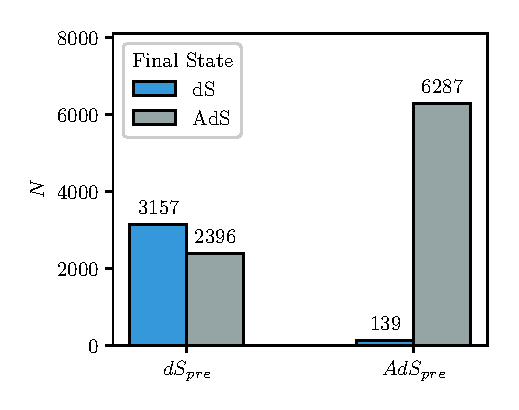
\includegraphics[width=\linewidth]{plots/transition_new.pdf}
\caption{Transition between vacuum types (new solutions).}
\label{fig:transition_new}
\end{minipage}
\hfill
\begin{minipage}{0.48\linewidth}
\centering
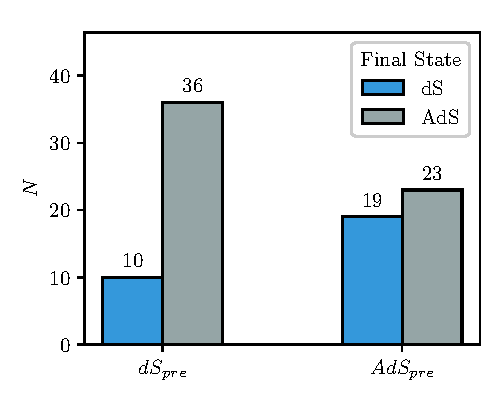
\includegraphics[width=\linewidth]{plots/transition_original.pdf}
\caption{Transition between vacuum types (original database).}
\label{fig:transition_original}
\end{minipage}
\end{figure}

\begin{figure}[htbp]
\centering
\begin{minipage}{0.48\linewidth}
\centering
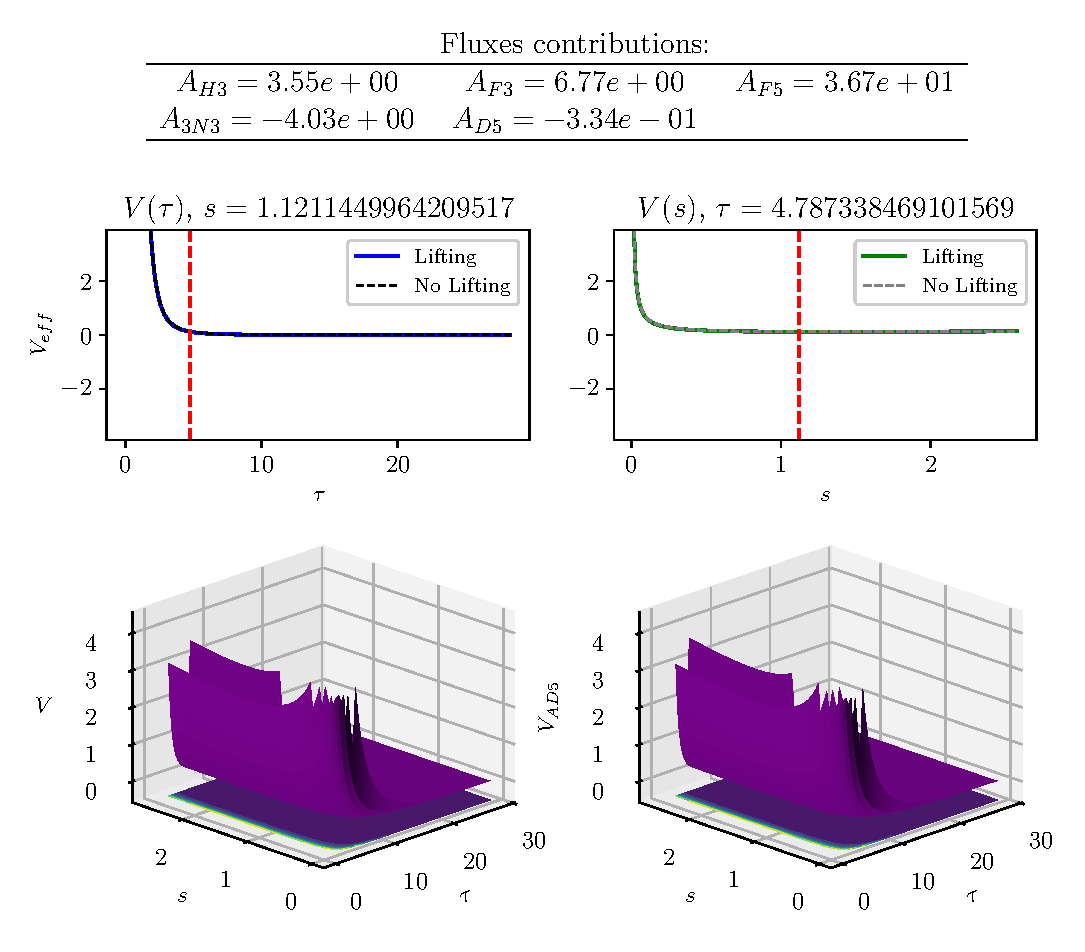
\includegraphics[width=\linewidth]{plots/stUnchanged.pdf}
\caption{A point that retained its vacuum type across the
         non‑lifted and lifted potentials.}
\label{fig:stUnchanged}
\end{minipage}
\hfill
\begin{minipage}{0.48\linewidth}
\centering
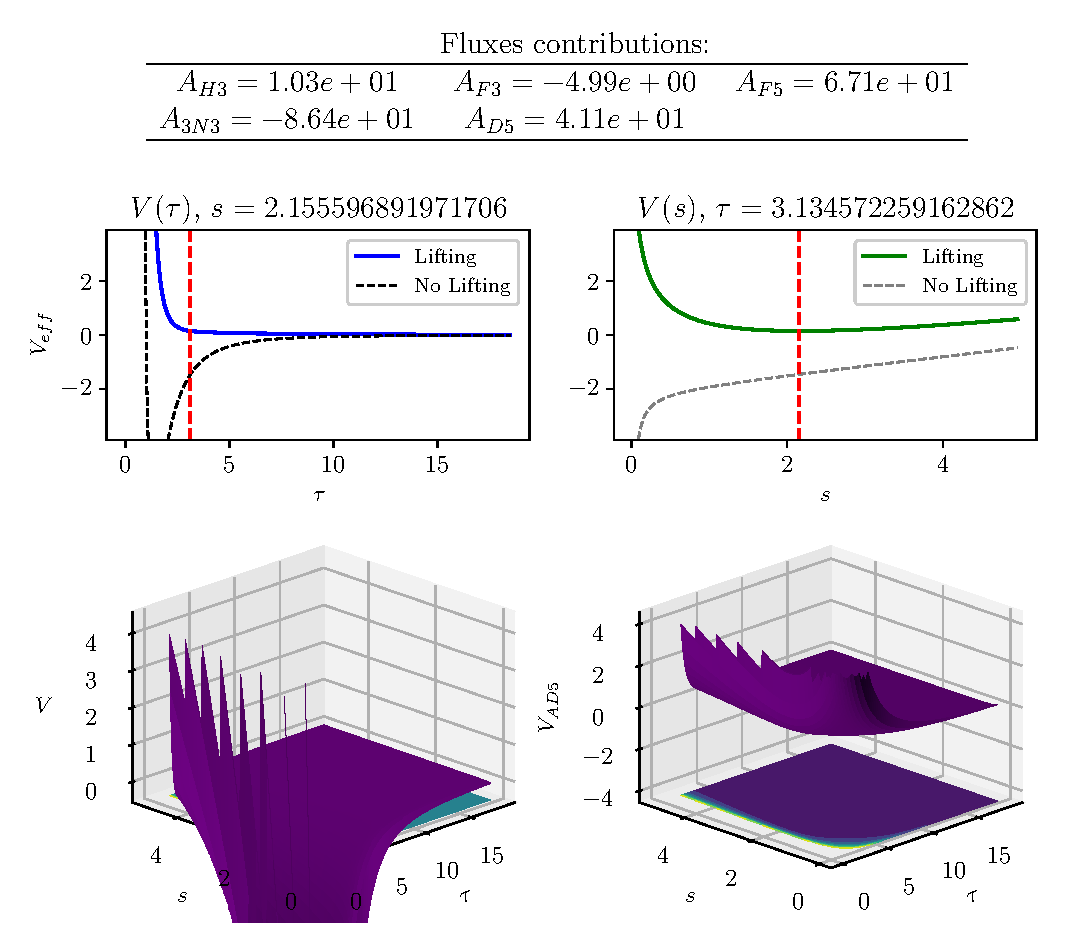
\includegraphics[width=\linewidth]{plots/AdS2dS.pdf}
\caption{Transition from anti‑de~Sitter to de~Sitter after
         lifting.}
\label{fig:AdS2dS}
\end{minipage}
\end{figure}
\begin{figure}[htbp]
\centering
\begin{minipage}{0.48\linewidth}
\centering
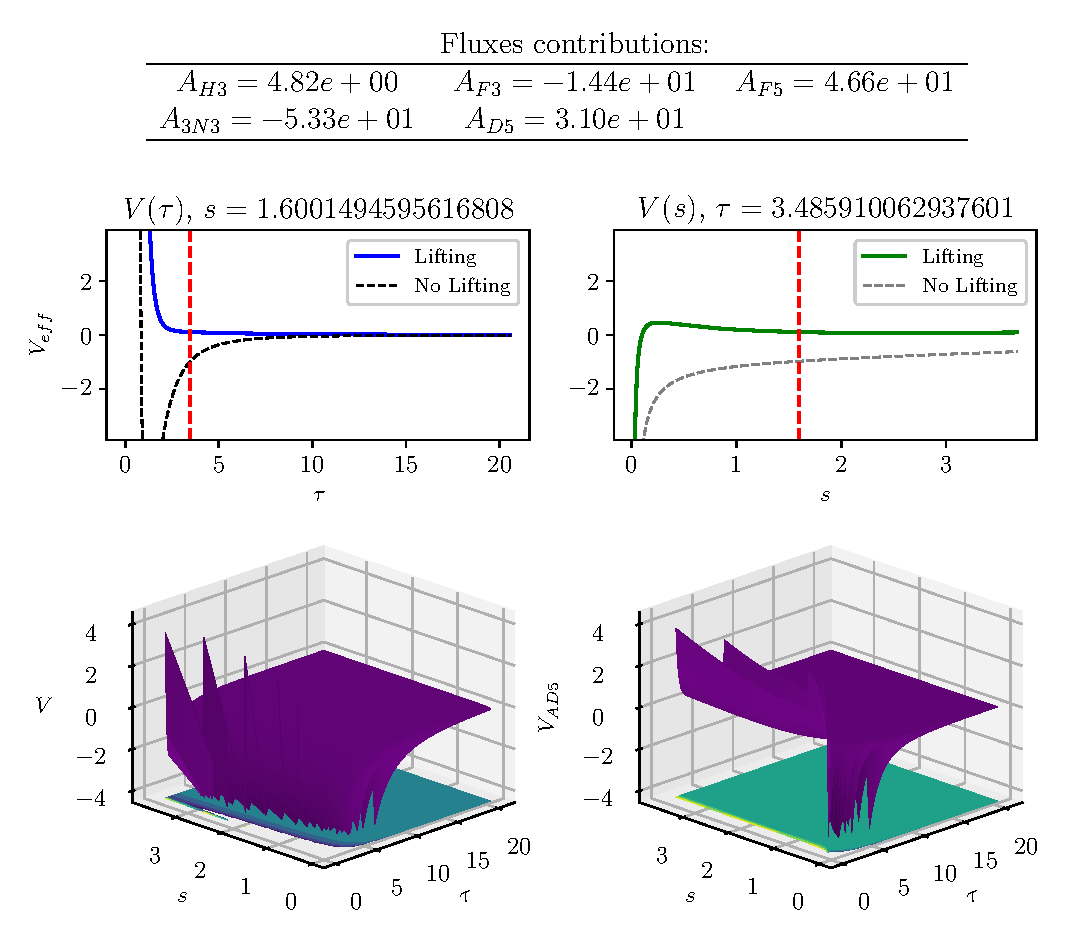
\includegraphics[width=\linewidth]{plots/sLifted.pdf}
\caption{Lifting acting primarily on the dilaton $s$.}
\label{fig:sLifted}
\end{minipage}
\hfill
\begin{minipage}{0.48\linewidth}
\centering
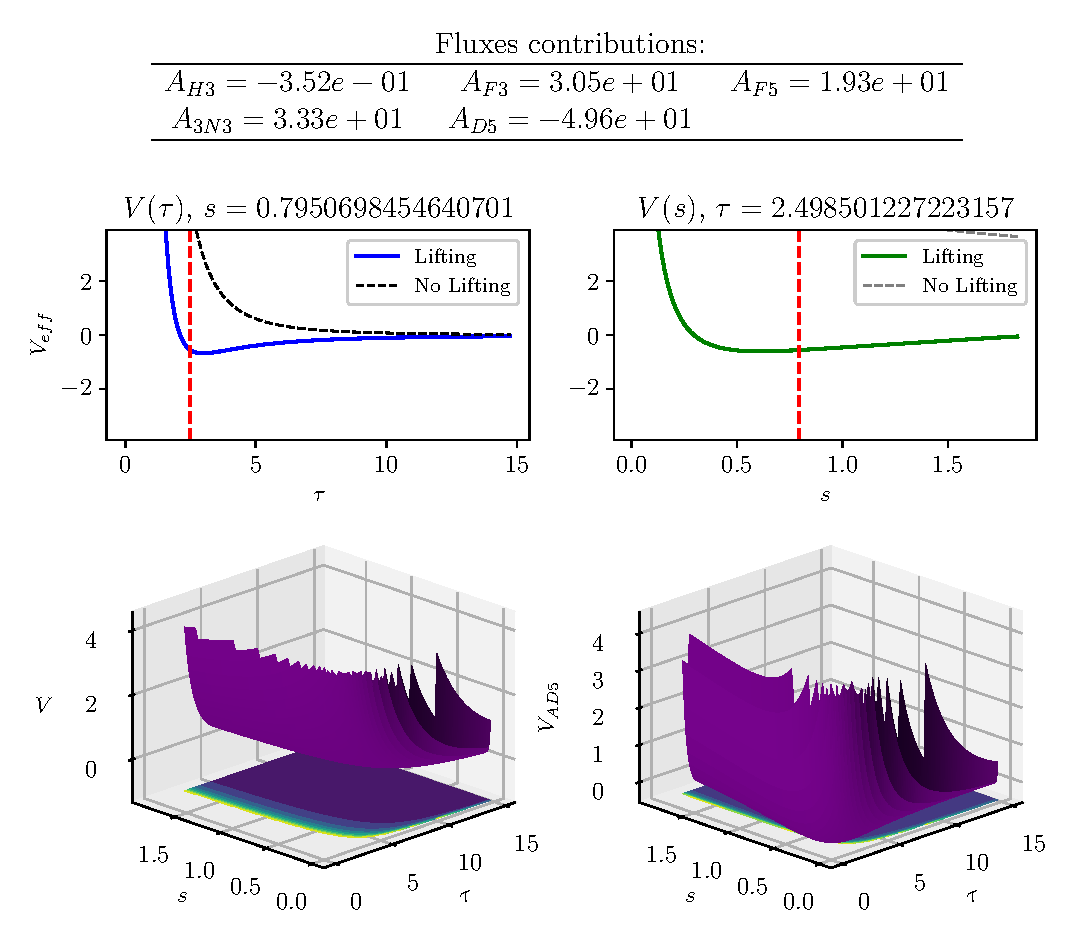
\includegraphics[width=\linewidth]{plots/stLowered.pdf}
\caption{Lowering of the potential along the moduli directions
         after lifting, leading to negative regions or
         flattening.}
\label{fig:stLowered}
\end{minipage}
\end{figure}

\subsubsection{Consistent Orientfolds Contribution ($A_3N_3$) Behaviour}
A noteworthy observation concerns the coefficient
$A_3\mathcal{N}_3$. Even though no sign restriction was imposed
during optimisation, the genetic algorithm consistently returned
negative values for this coefficient, in agreement with the
physical expectation.



\subsection{Grid experiment}
For further analysis an experiment was done regaring a grid of
\texttt{Basic GA} configurations. Originally the grid was planned
for around 800 different configurations.

\begin{itemize}
    \item \textbf{Epoch:} [50, 100, 200, 300, 400]
    \item \textbf{Population Size (pop\_size):} [20, 60, 100, 140, 180, 220, 260, 300]
    \item \textbf{Crossover Probability (pc):} [0.1, 0.3, 0.5, 0.7, 0.9]
    \item \textbf{Mutation Probability (pm):} [0.2, 0.4, 0.6, 0.8]
\end{itemize}

For testing different models, there were 6 different instances
of testing implementing different variations from which those
analysed were shown in the table~\ref{tab:detailed_parameters}.
The test was done over three different moduli configurations shown in
the table~\ref{tab:comparison_example}.

\begin{table}[h]
    \small
    \centering
    \caption{Detailed Parameters for Each Model}
    \label{tab:detailed_parameters}
    \renewcommand{\arraystretch}{1.3} % Adjust row spacing if needed
    \begin{tabular}{p{2cm} p{2cm} p{2cm} p{2cm} p{2cm}}
        \hline
        & \textbf{Epoch} & \textbf{Population Size (\(pop\_size\))} & \textbf{Crossover Probability (\(pc\))} & \textbf{Mutation Probability (\(pm\))} \\
        \hline
        Model 1 & 50 & 20 & 0.1 & 0.2  \\
        Model 2 & 100 & 60 & 0.9 & 0.8 \\
        Model 3 & 50 & 20 & 0.5 & 0.6  \\
        Model 4 & 50 & 60 & 0.5 & 0.6  \\
        \hline
    \end{tabular}
\end{table}

\begin{table}[h]
\centering
\caption{Moduli configurations ($s, \tau$) for the three experimental runs.}
\label{tab:moduli_configs}
\begin{tabular}{@{} l c c @{}}
    \hline
    \textbf{Configuration} & \textbf{$s$} & \textbf{$\tau$} \\
    \hline
    Run 1 & 1.600149459561681 & 3.485910062937601  \\
    Run 2 & 2.459242111292193 & 3.0947272010640288 \\    
    Run 3 & 1.053781742958659 & 1.4533862399266009 \\
    \hline
\end{tabular}
\end{table}

\subsection{Results of the grid}

\subsubsection{Stability of vacua}

For each model and each run, the fraction of stable vacua was computed.
Table~\ref{tab:stability_ratios} reports these stability ratios.

\begin{table}[h]
\centering
\caption{Stability ratios (stable vacua / total points) per model and run.}
\label{tab:stability_ratios}
\begin{tabular}{l c c c}
\hline
\textbf{Model} & \textbf{Run 1} & \textbf{Run 2} & \textbf{Run 3} \\
\hline
Model 1 & 0.49 & 0.31 & 0.87 \\
Model 2 & 0.44 & 0.17 & 0.99 \\
Model 3 & 0.50 & 0.36 & 0.96 \\
Model 4 & 0.43 & 0.25 & 0.98 \\
\hline
\end{tabular}
\end{table}

Model~3 exhibits consistently moderate‑to‑high stability, reaching
96\,\% in Run~3.

\subsubsection{Normality assessment}

Because later statistical tests require normality or lack thereof,
a Shapiro–Wilk test was applied to the distributions of the potential
\textbf{\(V\)} and the \textbf{fitness} metric for every combination
(Model, Run). Table~\ref{tab:normality_results} summarises the
outcomes (p‑values and decision at \(\alpha = 0.05\)).

\begin{table}[h]
\centering
\caption{Shapiro–Wilk normality test results for \(V\) and fitness.}
\label{tab:normality_results}
\small
\begin{tabular}{l l c c c l}
\hline
\textbf{Model} & \textbf{Run} & \multicolumn{2}{c}{\(V\)} & \multicolumn{2}{c}{fitness} \\
\cline{3-6}
& & p-value & normal? & p-value & normal? \\
\hline\\[-7pt]
1 & 1 & 0.0001 & No  & 0.1046 & Yes \\
1 & 2 & 0.0007 & No  & 0.0000 & No  \\
1 & 3 & 0.1623 & Yes & 0.0000 & No  \\
2 & 1 & 0.0000 & No  & 0.3620 & Yes \\
2 & 2 & 0.0036 & No  & 0.0719 & Yes \\
2 & 3 & 0.3750 & Yes & 0.3386 & Yes \\
3 & 1 & 0.0001 & No  & 0.5932 & Yes \\
3 & 2 & 0.0003 & No  & 0.0248 & No  \\
3 & 3 & 0.3651 & Yes & 0.0000 & No  \\
4 & 1 & 0.0000 & No  & 0.6264 & Yes \\
4 & 2 & 0.0042 & No  & 0.2522 & Yes \\
4 & 3 & 0.3894 & Yes & 0.0284 & No  \\[2pt]
\hline
\end{tabular}
\end{table}

Since many distributions deviate from normality,
non‑parametric tests were adopted for group comparisons.

\subsubsection{Statistical comparison of models}

For each of the three moduli groups (Run~1, Run~2, Run~3) the four
models were compared using the \textbf{fitness} metric.  Because the
data are not always normal, a Mann–Whitney \(U\) test was applied.
To keep the family‑wise error rate under control, the significance
level was adjusted with a Bonferroni correction: for three pairwise
comparisons per group, \(\alpha_{\text{corrected}} = 0.05 / 3 = 0.0167\).

Within each group the model with the highest median fitness was
selected as the candidate “best” model and then tested against the
other three.

\begin{table}[h]
\centering
\caption{Median fitness values and pairwise comparison results.}
\label{tab:statistical_comparison}
\begin{tabular}{c c c l}
\hline
\textbf{Run} & \textbf{Best Model} & \textbf{Median fitness} & \textbf{Outcome vs others} \\
\hline
1 & 3 & 0.1215 & Statistically better than Model~1 (p=0.0044), \\
     &      &        & Model~2 (p=0.0000) and Model~4 (p=0.0000). \\
     &      &        & \textbf{Clear winner.} \\
\hline
2 & 3 & 0.1560 & No statistical lead over Model~1 (p=0.0552); \\
     &      &        & better than Model~2 (p=0.0000) and \\
     &      &        & Model~4 (p=0.0000). \\
     &      &        & \textbf{Tie with Model~1.} \\
\hline
3 & 3 & 20.4978 & Statistically better than Model~1 (p=0.0002), \\
     &      &        & Model~2 (p=0.0000) and Model~4 (p=0.0000). \\
     &      &        & \textbf{Clear winner.} \\
\hline
\end{tabular}
\end{table}

\subsubsection{Visualisation of distributions}

Figure~\ref{fig:violin_plots} shows violin plots comparing the
potential \(V\) (upper panel) and the fitness (lower panel) across
the four models, with each run shown as a different colour.  
The plots confirm the spread and central tendency differences
observed in the statistical tests. And also a comparative histogram 
of stable vacua found during the grid is shown in figure~\ref{fig:stability_bar}.

\begin{figure}[htbp]
\centering

\includegraphics[width=0.9\textwidth]{plots/StabilityAnalysis.eps}
\caption{Number of stable vacua found by each model in each run of the grid analysis.}
\label{fig:stability_bar}

\includegraphics[width=0.9\textwidth]{plots/ViolinAG_comparison.eps}
\caption{Comparison of \(V\) (top) and fitness (bottom) across the four models.
Each model is shown with its three independent runs.}
\label{fig:violin_plots}
\end{figure}

\subsection{Challenges and Study Limitations}
\subsubsection{Behaviour Plotting} For some vacua found, the
potential behaviour could not be plotted due to unknown reasons.
Some suspects points towards numerical inconsistencies, asymptotic
range of moduli values, or equipment limitations. The main reason
to believe the points found and evaluated within the potential
are actually valid is that each point evaluated in both versions
of the potential exists.

\subsubsection{Time Limitations}
Some models were quite extensive, and due to the complexity of
the penalty function, even with GPU integration, their execution
times were still in the order of days. Instabilities on the
electrical service rendered these more complex models unfinished,
although they seemed to perform slightly better at first sight
based on some solutions noted in the logs.

\subsection{Conclusions}

The present work extended the analysis originally reported in
\cite{Damian2022} by replacing the simulated annealing and
conjugate gradient optimisation with a simple genetic algorithm
(GA). The search space was reformulated as a penalty‑based
optimisation over the five flux coefficients
\(A_{H_3},A_{F_3},A_{F_5},A_3\mathcal{N}_3,A_{\widehat{D5}}\),
each bounded uniformly to \([-100,100]\). This computational
approach allowed a more extensive exploration of the effective
potential landscape for type~IIB compactifications with torsion,
yielding a total of 11~979 critical points.

The results confirmed the capability of the GA to discover
stable de~Sitter vacua, with counts comparable to those
reported in the reference study. More importantly, the
systematic comparison between the non‑lifted and lifted
potentials revealed several non‑trivial behaviours that had not
been characterised before. Among these were points that
retained or changed their vacuum type under lifting, cases
where the lifting acted predominantly on a single modulus
(volume \(\tau\)), and configurations in which
the potential became significantly flatter or even developed
negative regions after lifting.

Even though no sign restriction was imposed on
\(A_3\mathcal{N}_3\), the GA consistently returned negative
values for this coefficient, in agreement with the physical
expectation. This observation suggests that the penalty‑based
formulation did not force artificial sign choices but allowed
the algorithm to converge to physically plausible regions.

Is also worth to mention that the exploitation of moduli
configurations is of special interest because of the
conjectures given by the swampland project.

A small fraction of the computed points exhibited numerical
instabilities that prevented their inclusion in the graphical
analysis. These points are mathematically valid but require
higher precision or alternative algebraic handling; their study
could uncover further structures of interest both from a
computational and from a string‑theory perspective.

On the other hand, the grid analysis found that tuning the
\texttt{GA} can give better results even with a basic
version of the algorithm.

Future work will extend the methodology to a wider family of
nature‑inspired algorithms (e.g. ant colony optimisation,
estimation of distribution algorithms, weed distribution
optimisation, atom search optimisation) to assess whether
alternative search strategies can further improve the
exploration of the landscape.

\begin{credits}
\subsubsection{\ackname}
The first author acknowledges the support from CONAHCYT (now
SECIHTI) for the master's scholarship (CVU: 1295151).

\subsubsection{\discintname}
The authors have no competing interests to declare that are relevant
to the content of this article.
\end{credits}
%
% ---- Bibliography ----
%
% BibTeX users should specify bibliography style 'splncs04'.
% References will then be sorted and formatted in the correct style.
%
\bibliographystyle{splncs04}
\bibliography{bib}


\end{document}
